\setcounter{chapter}{12}
\chapter{Programowanie miktrokontrolerów i mikroprocesorów}
\PartialToc
%\startcontents[chapters]
%\printcontents[chapters]{}{1}{\section*{\contentsname}}
\setcounter{section}{215}

%-----------------
\answer
{Ile rejestrów 8-bitowych dostępnych dla programisty znajduje się w procesorach z rodziny x86?}
{6}
{F}
{8}
{
	Innej poprawnej nie ma. Rysunek poniżej
	\begin{center}
		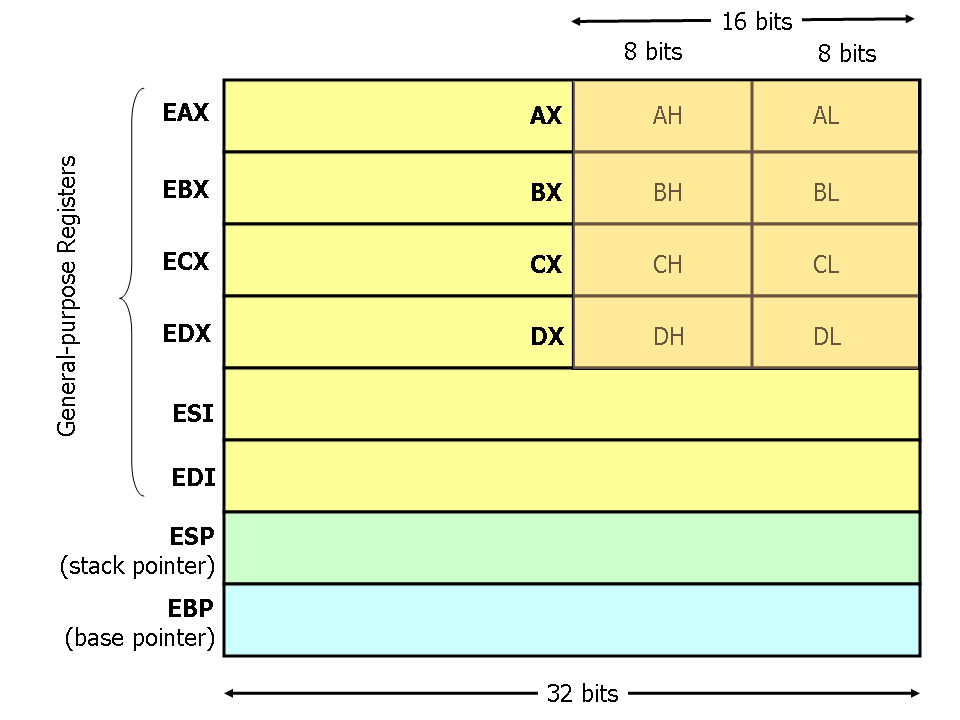
\includegraphics[width=6cm]{13/img/x86-registers.png}
		\captionof{figure}{Struktura rejestrów procka x86}
	\end{center}
}
%-----------------
\answer
{Jaki tryb adresowania wykorzystuje rozkaz ADDL (\%ebx),\%eax?\\}
{bezposredni}
{F}
{pośredni}
{
	Główny podział:
	\begin{itemize}
		\item bezpośredni (ang. direct)
		\item pośredni (ang. indirect)
	\end{itemize}
	Bardziej szczegółowo:
	\begin{itemize}
		\item rejestrowy (ang. register)
		\item rejestrowy pośredni (ang. register indirect)
		\item z przesunieciem (indeksowanie) (ang. displacement (indexed))
		\item stosowy (ang. stack)
	\end{itemize}
}
\begin{lstlisting}
bezposredni
movl 0x01, %eax
posredni
movl (%ebx), %eax
movl (%esi,%edi,1), %eax

\end{lstlisting}
%-----------------
\answer
{Jaka instrukcja jest równowazna w działaniu do instrukcji SHL \$1,\%eax?}
{SAL \$1,\%eax}
{T}
{}
{\\\textbf{SAL} - przesunięcie arytmetyczne w lewo\\
	\textbf{SHL} - przesunięcie bitowe w lewo.\\
	Przesuwanie w lewo czyli w stronę flagi CF. Przy ostatnim przesunięciu flaga zostanie wyzerowana więc nie ma znaczenia dla wyniku czy stosujemy arytmetyczne czy bitowe przesuniecie.}
\begin{lstlisting}
MOVW $0xFF00, %ax   #=> 0xff00 65280   # 1 1111 1111 0000 0000
SHL   $1, %eax      #=> 0x1fe00 130560 # 1 1111 1110 0000 0000
##
MOVW $0xFF00, %ax   #=> 0xff00 65280   # 1 1111 1111 0000 0000
SAL   $1, %eax      #=> 0x1fe00 130560 # 1 1111 1110 0000 0000

\end{lstlisting}
%-----------------%-----------------
\answer
{Która z ponizszych instrukcji dotyczy operacji na blokach danych?}
{STC}
{F}
{np. \textbf{MOV, PUSH, POP, XCHG, XLAT}}
{\begin{itemize}
		\item[] \textbf{STC} (STC/CLC - set carry / clear carry. Do flagi CF wstaw 1 lub 0, odpowiednio). \\FLAGI: \textbf{CF, OF, SF, ZF, IF, PF, DF} służą przede wszystkim do sterownia znacznikami np. do badania wyniku ostatniego przekształcenia (przepełnienie / wynik 0).
	\end{itemize}}
	%More - wykłądy Bublińskiego, Język asembler dla każdego Bogdan Drozdowski
	%-----------------%-----------------
	\answer
	{Według jakiej reguły moze być dokonywana konwersja do liczby całkowitej w jednostce FPU (Floating Point Unit)?
	}
	{round down}
	{T}
	{\\
		00 - round to nearest\\
		01 - round down\\
		10 - round up\\
		11 - round toward zero\\}
	{Powyżej możliwe ustawienia kontroli zaokrągleń w FPU. \\Źródło wykłady FTP wykłd 9. s16}
	%-----------------%-----------------
	\answer
	{Ile razy wykona sie pętla zbudowana w oparciu o instrukcję LOOP, jesli przed jej rozpoczeciem zawartosc rejestru \%ecx była równa 0? }
	{$2^{32}$}
	{T}
	{Chyba poprawne?}
	{rozkaz loop to petla for(\%ecx - -;\%ecx!=0;)\{\%ip+=disp\}. \\Źródło wykłady FTP}
	%-----------------%-----------------
	\answer
	{Ile razy zawartosc rejestru \%ah zostanie zapisana do pamieci poprzez uzycie instrukcji REP STOSB, jezeli przed jej wykonaniem zawartosc rejestru \%ecx była równa x?}
	{1}
	{F}
	{hmm czyżby chodzilo o zawartość al?, jeśli nie to zero razy bo STOSB wpisze AL nie AH, a jesli mial na mysli AL to x razy}
	{REP powtarza instrukcje x razy, w tym wypadku wezmie pod uwage rejestr CL jako licznik}
	%-----------------%-----------------
	\answer
	{
		Jaka bedzie zawartosc rejestru \%eax po sekwencji rozkazów?\\
		MOVL \$0xFFFF0000 ,\%eax\\
		NEG \%eax
	}
	{0x00000000}
	{F}
	{0x00010000}
	{
		\lstinputlisting{13/ideone_5Uwlpn.s}
	}
	%-----------------%-----------------
	\answer
	{Jaka bedzie zawartosc rejestru \%al po sekwencji rozkazów? \\
		MOVW \$0xFF00 ,\%ax\\
		ADCB \%ah ,\%al\\
		ADCB \%ah ,\%al\\
	}
	{nieokreslona}
	{F}
	{0xFFFE}
	{
		\lstinputlisting{13/ideone_13223.s}
	}
	%-----------------%-----------------
	\answer
	{Na jakim rodzaju schematu pokazane sa połaczenia elektryczne w układzie opartym na mikrokontrolerze?}
	{ideowym}
	{T}
	{?}
	{}
	%-----------------%-----------------
	\answer
	{W jakim rodzaju pamieci mikrokontrolera uzytkownik zwykle zapisuje kod programu?}
	{DRAM}
	{F}
	{
		\begin{itemize}
			\item EEPROM, Flash - zwykle
			\item EPROM, MRAM lub FRAM
		\end{itemize}
	}
	\\{Powyżej wymienione pamięci są pamięciami nieulotnymi, i tam umieszczamy kod programu.\\DRAM i SRAM są pamięciami ulotnymi, czyli po wyłączeniu zasilania kod przepada.}
	%-----------------%-----------------
	\answer
	{Jakie elementy wystepujace w mikrokontrolerach nie wystepuja w mikroprocesorach?}
	{ADC}
	{T}
	{}
	{\begin{itemize}
			\item Mikroprocesor to tylko:\\- \textbf{ALU} (Arithmetic Logic Unit) - jednostka licząca\\ - \textbf{CU} (Control Unit) - układ sterujący pracą\\ - \textbf{Rejestry}: PC, IR, SP - potrzebne przy wykonywaniu operacji obliczeniowych\\
			\item Mikrokontroler to układ w pełni autonomiczny, potrzebujący tylko zasilanie do pracy. Posiada w sobie procesor oraz peryferia np.:\\- pamięć danych do przechowywania kodu programu i zmiennych,\\- porty wejścia-wyjscia np: \textbf{ADC} (Analog-to-digital converter), \textbf{DAC},\\- układy czasowo-licznikowe, \\- kontrolery przerwań,\\- kontrolery transmisji\textbf{ UART, SPI, I2C, USB, CAN, 1-Wire} etc.,\\- zegar czasu rzeczywistego \textbf{RTC},\\- watchdog.
		\end{itemize}}
		%-----------------%-----------------
		\answer
		{Czy jezyk maszynowy jest tozsamy z jezykiem asemblera? }
		{nie}
		{T}
		{}
		{Język ASM to tekstowe odpowiedniki wewnętrznych rozkazów procesora (tzw. mnemoniki), kod maszynowy to po prostu liczby}
		%-----------------%-----------------
		\answer
		{Jakie narzedzie słuzy do zamiany kodu napisanego w jezyku asemblera na kod maszynowy? }
		{assembler}
		{T}
		{}
		{}
		%-----------------%-----------------
		\answer
		{Które z narzedzi nie umozliwia stworzenia kodu na mikrokontroler z rodziny AVR?}
		{Microsoft Visual Studio
		}
		{F}
		{Wszystkie narzędzia które nie wspierają Make, czyli da się np. w Eclipse, dedykowane do AVR jest AVR Studio}
		{http://www.instructables.com/id/Use-Visual-Studio-2010-to-Compile-AVR-Hex-Files/}
		%-----------------%-----------------